\section{Zeitplan}\label{zeitplan}
\begin{figure}[H]
	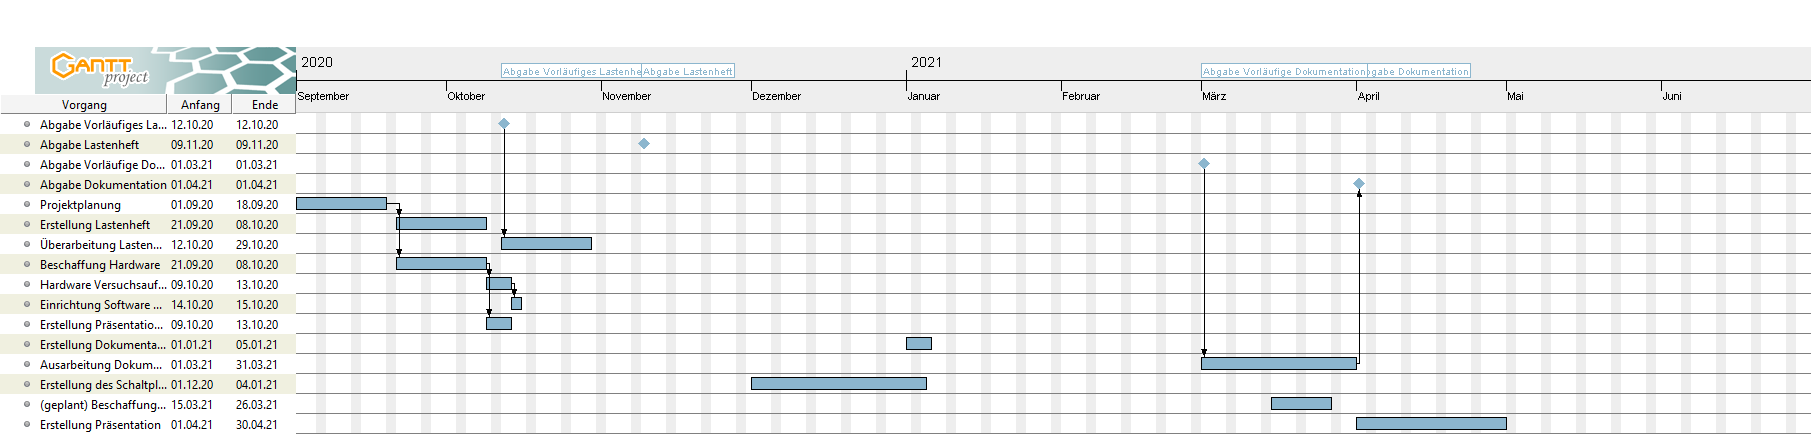
\includegraphics[width=1\textwidth]{img/TAR_FKMS_20202021.png}
	\caption[gantt-Diagramm des Projektablaufs]{gantt-Diagramm des Projektablaufs}
 	\label{fig:gantt-diagramm}
\end{figure}
Um einen besseren Überblick der Aufgaben zu haben, haben wir mit GanttProject ein Gantt-Diagramm mit den Aufgaben und Meilensteinen unseres Projekts angelegt (vgl. Abb. \ref{fig:gantt-diagramm}: \nameref{fig:gantt-diagramm}).
Die eigentliche Projektorganisation war als SCRUM Projekt geplant. Hierfür haben wir das KANBAN-Board in Microsoft Teams genutzt (vgl. Abb \ref{fig:kanban}: \nameref{fig_kanban}).
Dadurch haben wir stets einen Überblick über die noch zu erledigenden, offenen und erledigten Aufgaben.\\
\begin{figure}[H]
    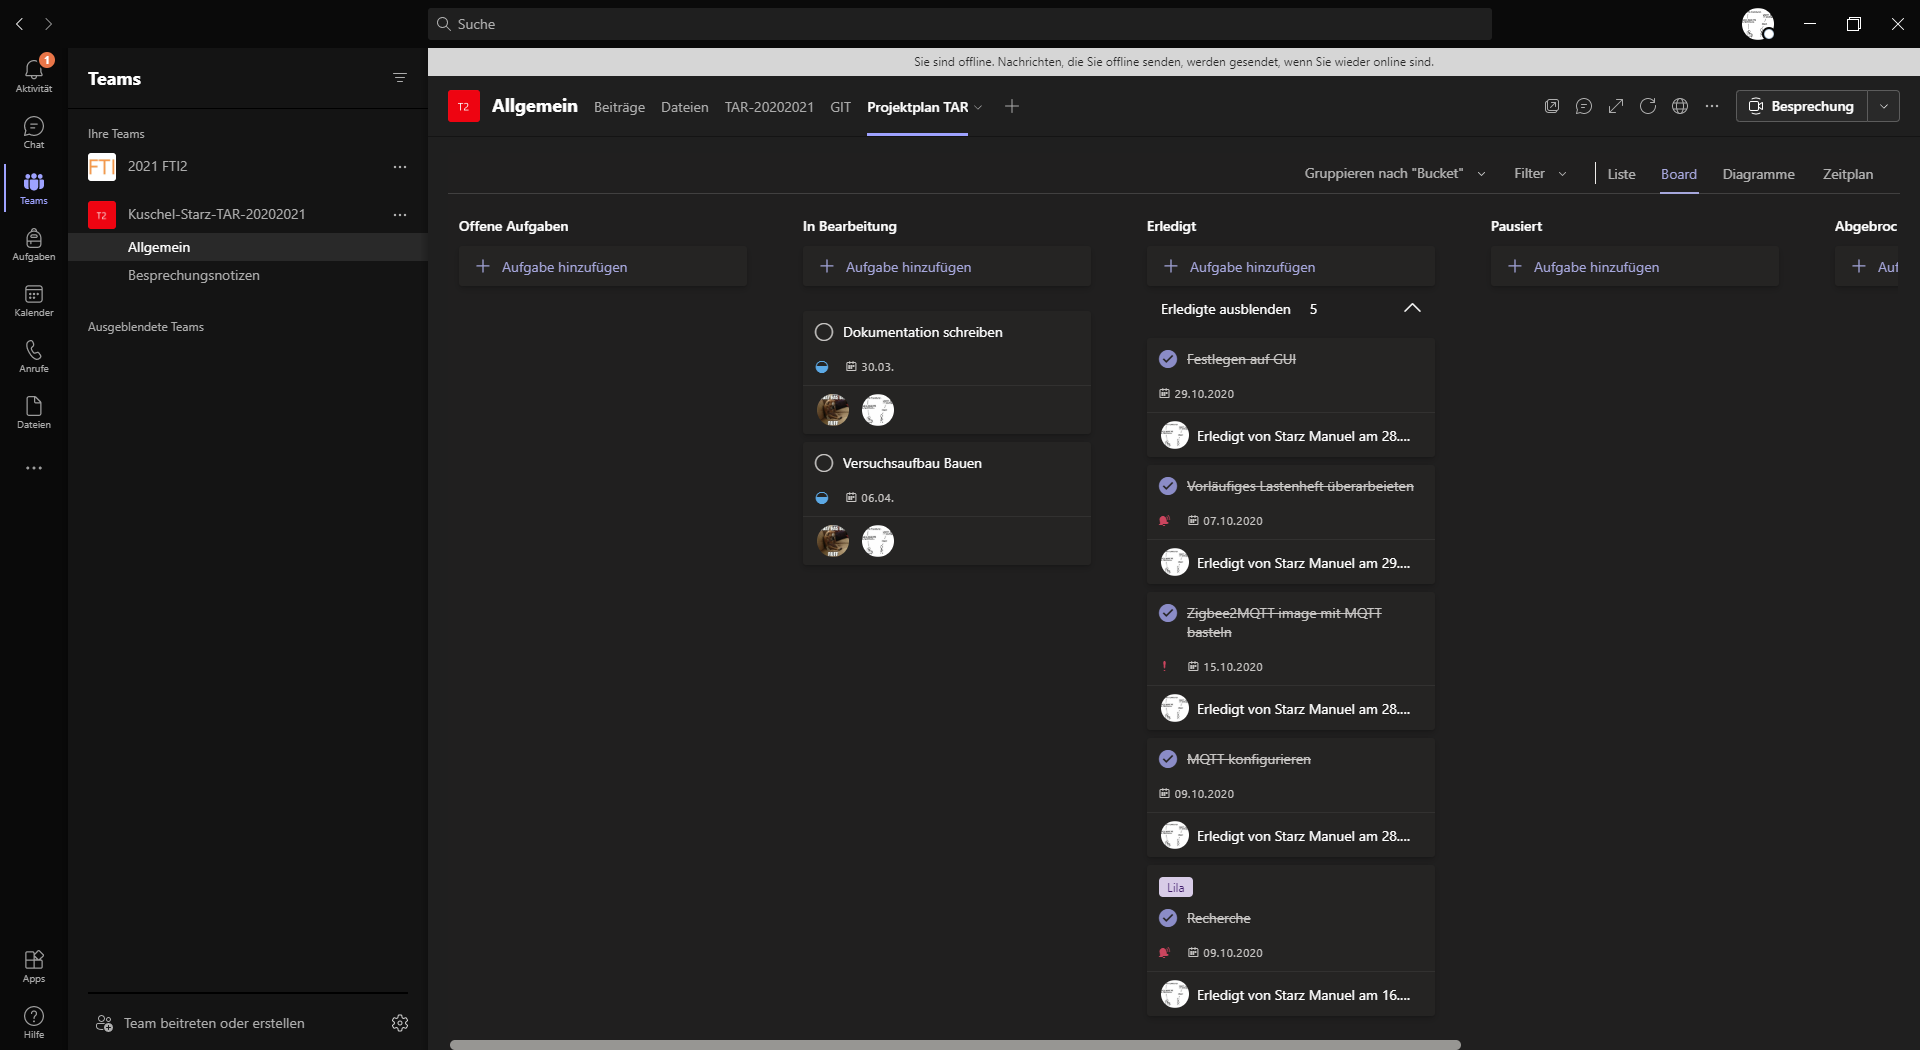
\includegraphics[width=1\textwidth]{img/teams_kanban.png}
    \caption[KANBAN-Board in Microsoft Teams]{KANBAN-Board in Microsoft Teams}
    \label{fig:kanban}
\end{figure}
\noindent Microsoft Teams hat uns auch als Kommunikationsplattform während der Lockdown-Zeiten. 
Dadurch konnten wir während der üblichen Zeiten mit Herr Kohler in Verbindung treten.
\newpage